\section{Introduction}
\label{sec:intro}

\begin{figure}[h]
    \centering
    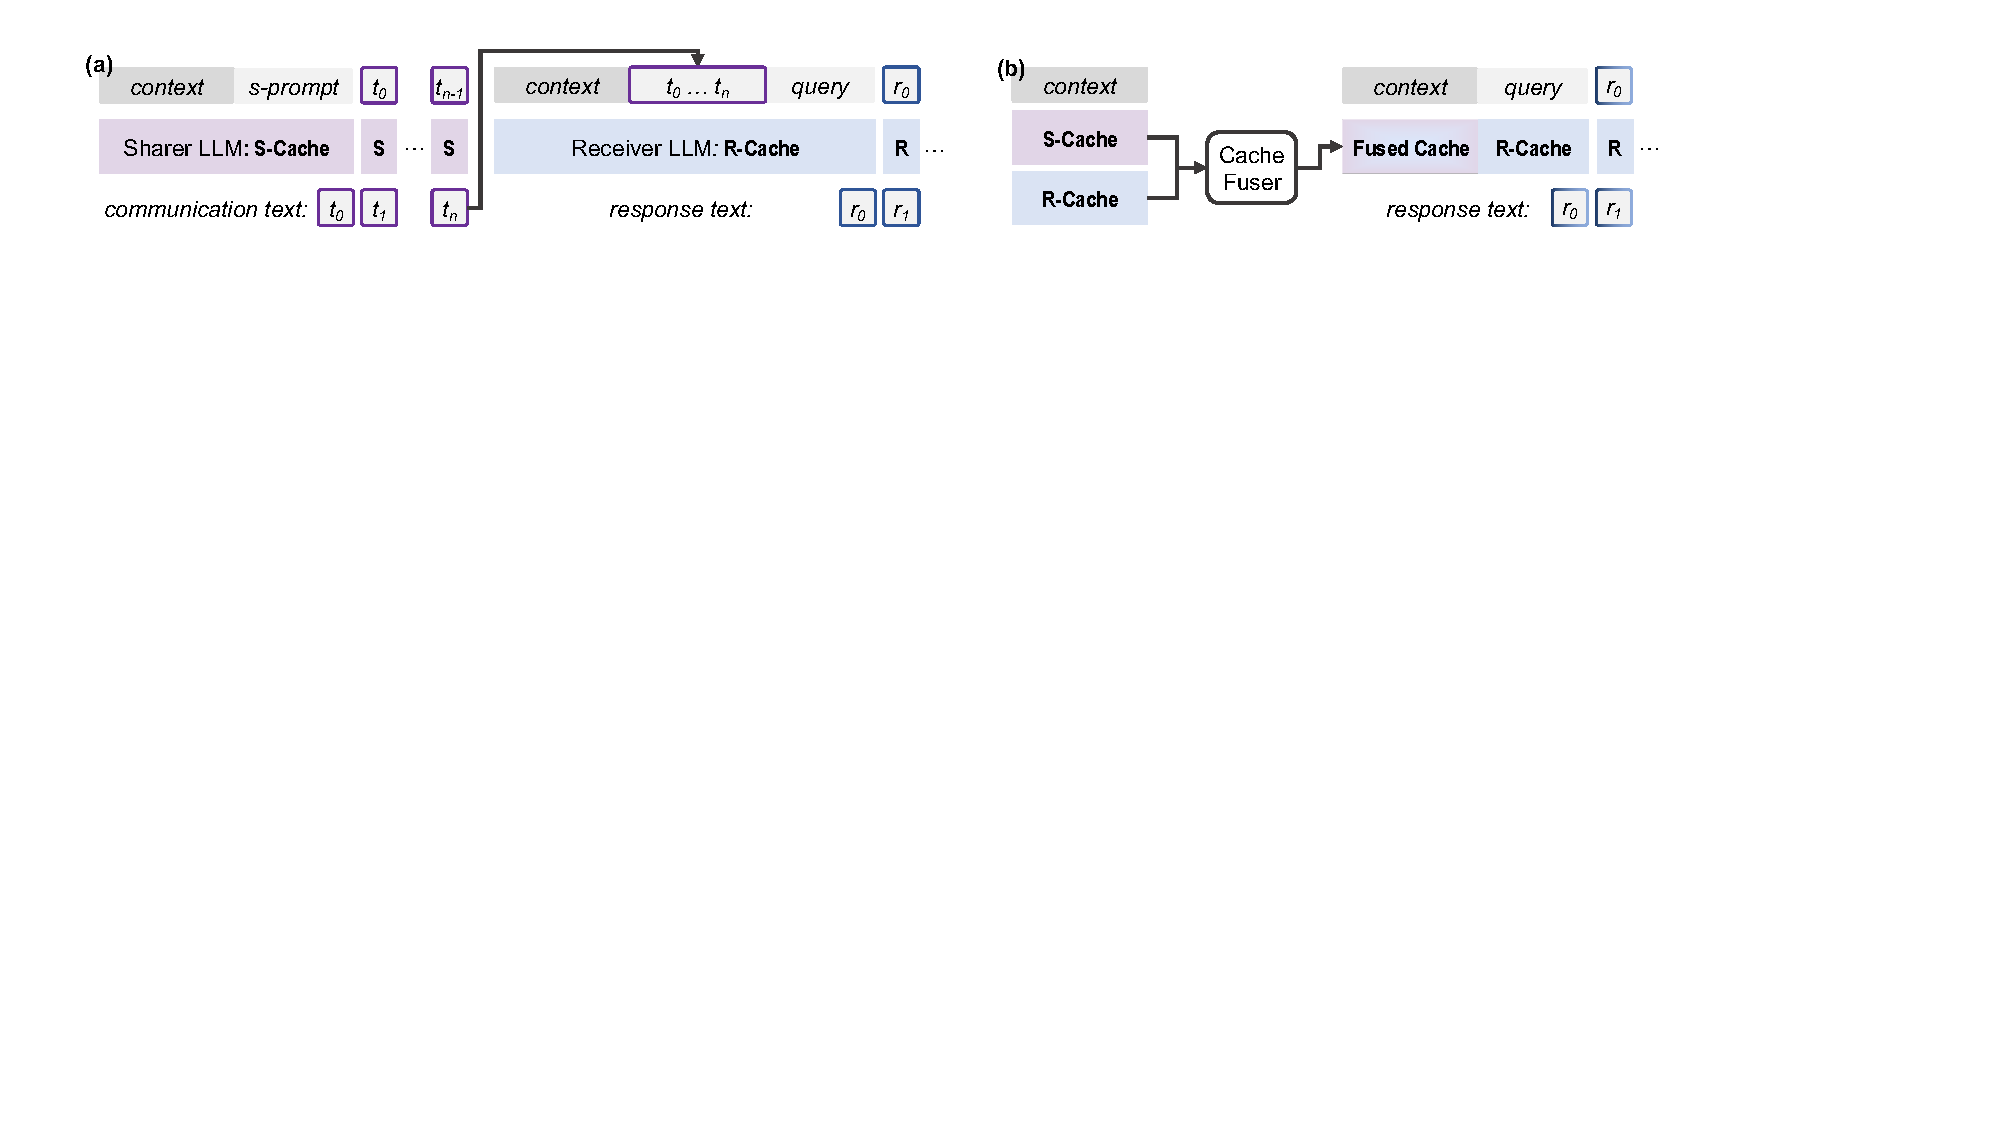
\includegraphics[width=\textwidth]{figure/scheme.pdf}
    \caption{(a) Previous Text-to-Text (T2T) communication passes information through explicit text generation. (b) Our Cache-to-Cache (C2C) communication directly projects and merges KV-Cache with rich semantics from different LLMs.}
    \label{fig:scheme}
\end{figure}

% “Our \name system enables direct cache-to-cache communication—akin to telepathic exchange of internal representations—allowing LLMs to collaborate without verbose text handovers.”

% We use 'semantic' to refer to the rich, meaning-bearing internal representations encoded in the KV-cache, which capture each model's unique understanding and interpretation of the input beyond surface-level text."

% What problem?
% Diverse LLMs
With the rapid progress of Large Language Models (LLMs)~\citep{guo2025deepseek-r1, yang2025qwen3, OpenAI2025GPT5}, they are now applied across increasingly diverse domains and tasks.
To meet versatile demands, LLMs are trained with distinct focuses, such as coding~\citep{hui2024qwen2.5-coder}, mathematics~\citep{yang2024qwen2.5-math}, visual understanding~\citep{bai2025qwen2.5-vl}, edge computing~\citep{zhang2024edgeshard}, and so on.
Meanwhile, general-purpose LLMs can also simulate specialized capabilities through prompt engineering, enabling flexible role adaptation across downstream applications.

% Muti-LLM system
% Why important problem?
% Model communication is important
% 1. Different LLMs have their respective strengths.
% 2. Privacy: cloud-edge collaboration
Leveraging the diversity of LLMs, many multi-LLM systems are proposed to further enhance overall performance and efficiency~\citep{guo2024agentsSurvey, tran2025collabSurvey}. 
% Multi-LLM collaborations
% Actively communicate; E.g., Camel, AutoGen
% by using different models or prompting.
In \textbf{collaborative multi-LLM systems}~\citep{li2023camel, wu2023autogen}, LLMs are assigned distinct roles and proactively exchange text messages.
Mirroring human collaboration, these systems accumulate partial understandings or sub-solutions from different agents via verbal communication. They harness the collective capabilities of multiple LLMs to solve complex problems that a single model cannot.
% Non-active communication, share context; E.g., speculative decoding, R2R, (query-level routing: model switching)
By contrast, \textbf{routing-based} multi-LLM inference systems rely on passive context inheritance rather than active message exchange.
These systems coordinate models of varying parameter sizes or reasoning depths for more dynamic and efficient responses~\citep{li2024eagle, fu2025r2r, ong2024routellm, OpenAI2025GPT5}.
Downstream models inherit the context from preceding models in multi-round conversations, then generate follow-up responses to the new questions based on their own understanding of the conversation history.

% Previous solutions
% Current works use a text interface.
% 1. Performance: Limited information exchange, limited to verbal text expressions, or entirely no communication
% 2. Efficiency: For active communication systems, they require an entire decoding stage to explicitly convey the understanding of the question in text.
% Future work: *Privacy, Explicit exchange of textual information that can be easily hacked.
However, current text-to-text (T2T) interfaces restrict information exchange among LLMs, particularly when conveying rich or diverse semantic interpretations of a shared context. 
As illustrated in Figure~\ref{fig:idea}, these limitations arise from several inherent constraints of T2T communication.
First, as a low-bandwidth medium, text introduces an information bottleneck. The high-dimensional internal representations must be repeatedly compressed into linear strings and then decompressed by the receiver LLM. 
When models differ in knowledge or assigned roles, some signals may be irrecoverable (e.g., interpreting \texttt{<p>} as a section marker).
Second, natural language is inherently ambiguous, with idioms, underspecified references, and vague expressions. 
Although recent agent protocols aim to standardize text messages~\citep{anthropic2024mcp, google2025a2a}, rigid templates remain insufficient for flexible, open-domain collaboration.
Third, T2T communication incurs noticeable latency. 
Every exchange requires exhaustive, token-by-token decoding of contextual explanations in sequence.
These limitations motivate a key question:
\highlightblock{Can LLMs communicate beyond text?}

% % What solutions?
% % Key insight / idea
% Challenge1: how to share deeper understanding efficiently beyond text}
% Challenge2:  what is the method: directly replace?}
% To explore this question, we focus on KV-Cache as a naturally richer representation than text.
% We find that enriching KV-Cache embeddings with additional few-shot semantics improves response accuracy by $3.92\%$ under the same context length and cache size (detailed in Section~\ref{sec:oracle}). 
% Moreover, despite comparable overall performance, 59.0-63.7\% of correctly answered questions differ between Qwen3-0.6B and Qwen2.5-Math-1.5B (Figure~\ref{fig:venn}).
% It shows that different LLMs encode distinct semantic understandings and contextual knowledge of the same input, reflecting their complementary strengths. 

% % Main idea: communication using KVCache
% % Method: Project KVCache from the source model to the target model and fuse them.
% Encouraged by these oracles, we propose Cache-to-Cache (\name), a new paradigm for richer and faster multi-LLM communication.
% As shown in Figure~\ref{fig:scheme}(b), \name projects the KV-Cache from a source model into the space of a target model and merges them through a neural Cache fuser.
% % Benefits
% % Performance: With richer semantics beyond the context itself. Harness internal understanding of LLMs, beyond the output texts.
% % Efficiency: High-parallelism, compared with token-by-token decoding (with explicit prompts) and sequential handover.
% Compared with T2T, \name communicates in the model’s internal representation space, conveying semantics beyond the explicit context.
% It also enables fully parallel communication through direct projection, avoiding the slow sequential decoding required in text exchanges.
% Our contributions are summarized as follows.

% % Main contributions
% \begin{itemize}
%     \item We propose \name, a novel multi-LLM communication paradigm. 
%     Compared with existing text-to-text communication, it conveys richer semantics without explicit intermediate token-by-token decoding.
%     \item We design and train the neural \emph{Cache fuser} to align and fuse KV-caches between models, leveraging their complementary semantic representations. 
%     \item  Experiments show that \name achieves 8.5-10.5\% higher average accuracy than individual models. It further outperforms the T2T paradigm by approximately 3.0-5.0\%, while delivering an average 2.0$\times$ speedup in latency.
% \end{itemize}

In this work, we explore using KV-Cache as the medium for LLM communication. 
KV-Cache is a naturally richer representation than text. It also enables fully parallel communication through direct projection, avoiding the slow sequential decoding in text exchanges.
Our oracle experiments show that
(1) enriching KV-Cache under the same context length increases accuracy,
(2) KV-Cache is convertible between LLMs, 
(3) different LLMs encode distinct semantic understandings and contextual knowledge of the same input, reflecting their complementary strengths.

Encouraged by these findings, we propose Cache-to-Cache (C2C), a new paradigm for richer and faster multi-LLM communication. As shown in Figure~\ref{fig:scheme}(b), \name projects the KV-Cache from a source model into the space of a target model and merges them through a neural cache fuser. 
Experiments show that \name achieves 6.4-14.2\% higher average accuracy than individual models. It further outperforms the T2T paradigm by approximately 3.1-5.4\%, while delivering an average 2.5$\times$ speedup in latency.

\begin{figure}[tb]
    \centering
    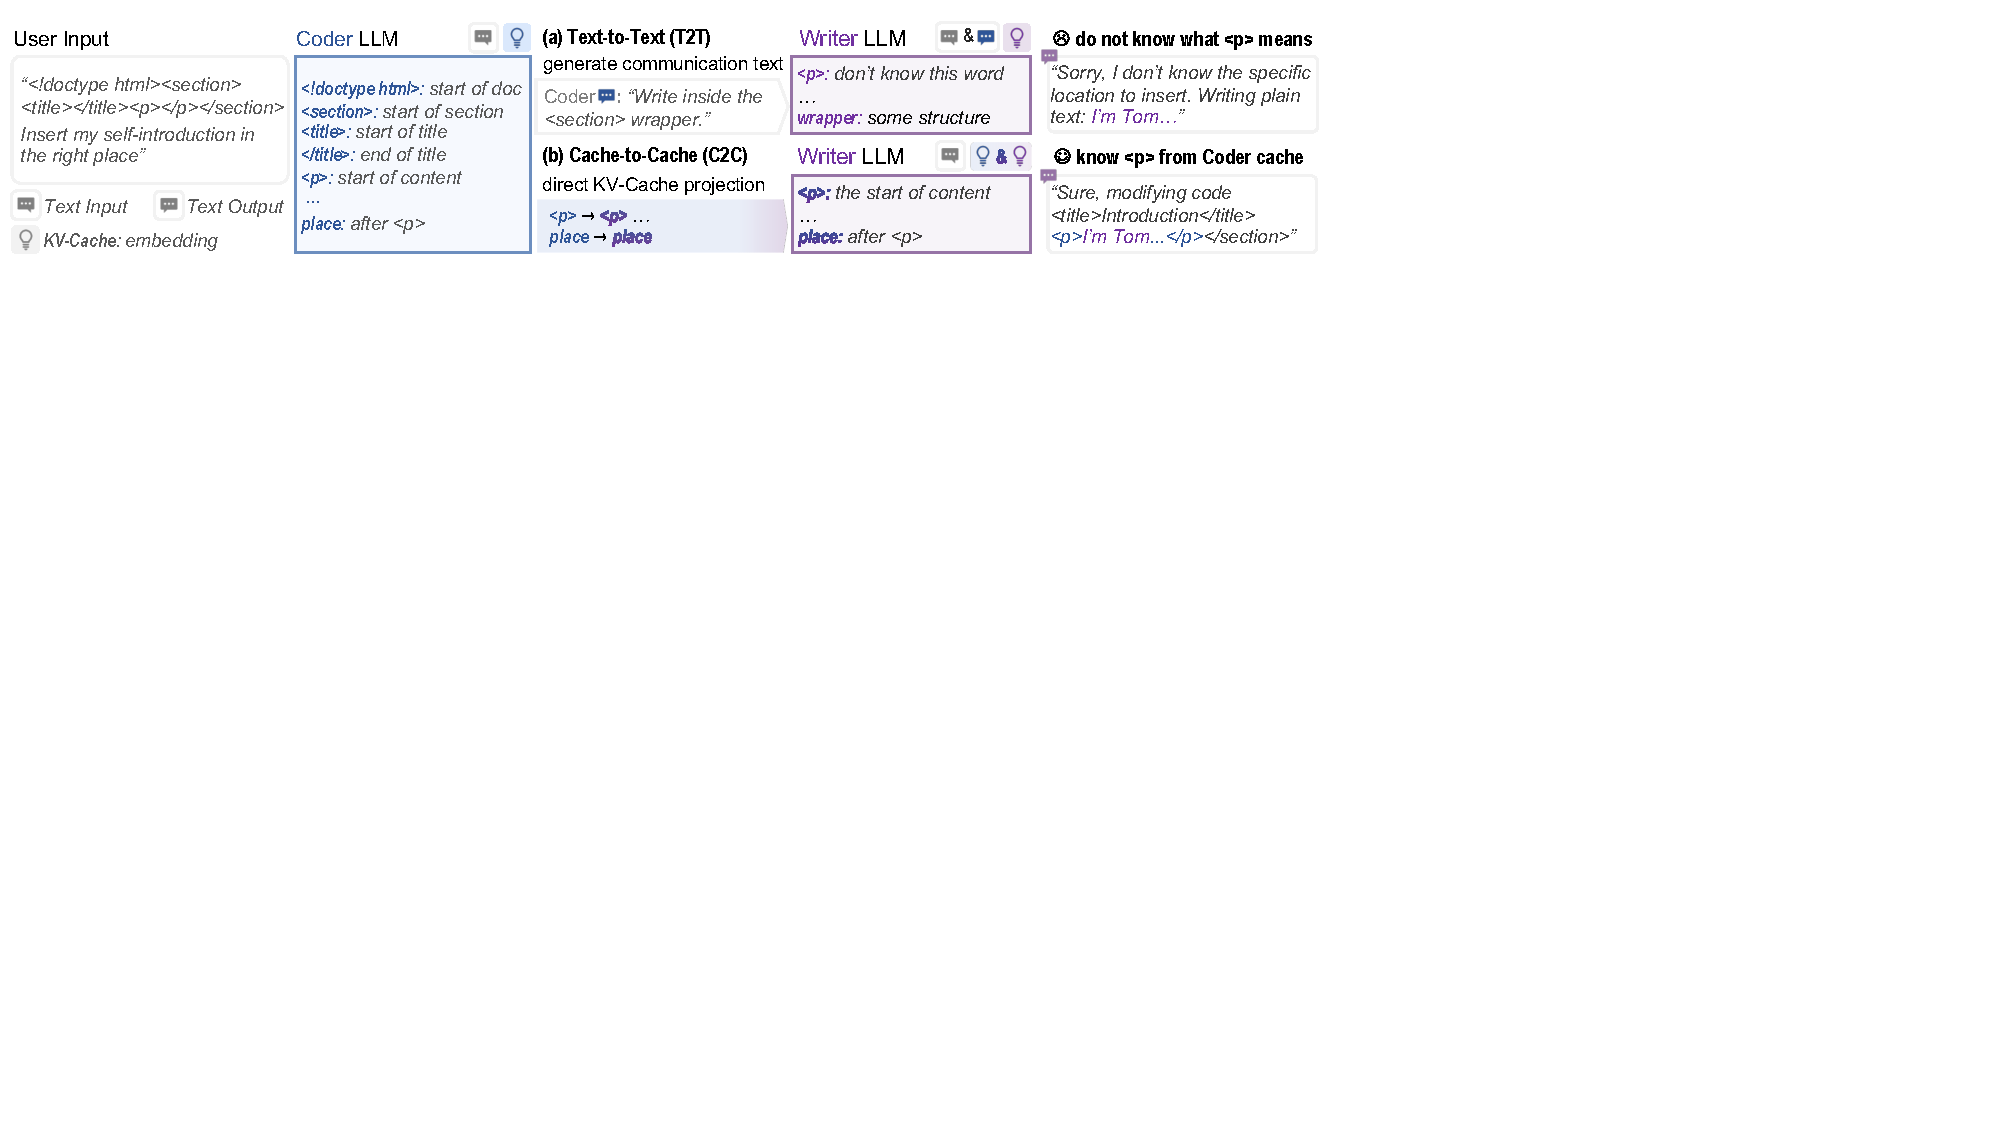
\includegraphics[width=\textwidth]{figure/idea.pdf}
    \caption{
    Conceptual comparison of T2T and C2C communication in a Coder-Writer collaboration example. 
    In T2T, the Coder's ambiguous text instruction fails to convey the structural semantics of \texttt{<p>} as a paragraph separator, causing the Writer to misplace the content. 
    \name directly projects the Coder's KV-Cache into the Writer, transferring both the semantic understanding and precise insertion location without intermediate text generation.
    }
    \label{fig:idea}
    \vspace{-8pt}
\end{figure}



